\problemname{Origami}

Filip found a pile of square origami papers. In preparation for
winter, and partly because he did not really know what origami is, he
decided to cut the papers into smaller pieces, place the pieces on the
blades of his ceiling fan, and turn the fan on. (He has a loft bed so
he can reach the ceiling fan easily.) As the pieces blew away, he
watched it ``snow'', over and over.

Now Filip is a little older, wiser, and he needs to clean his room. As
he is picking up the pieces of cut paper, he notices that there are
nice patterns on them. He sorts them by patterns and now he would like
to tape them back together the way they used to be. Each paper was a
square, though the squares were of several different sizes. The
trouble is, Filip is not sure if he found all the pieces! Help him
figure out whether he can form a square out of the pieces he got.

Each piece is a polygon (Filip is very proud of his straight-line
cutting abilities) and each piece originally touched the boundary of
the square. Filip remembers that he cut each square into at most 5
pieces. To form a square, the pieces cannot overlap. The patterns on
the pieces allow us to orient them so that it is sufficient to
consider only 90 degree rotations; however, you may need to flip some
pieces over.

\begin{figure}[h]
  \centering
  
\includegraphics{case1}
  \caption{Sample case 1.}
\label{fig:sample1}
\end{figure}
\begin{figure}[h]
  \centering
  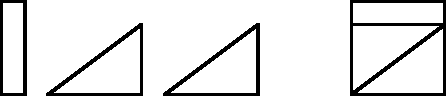
\includegraphics{case2}
  \caption{Sample case 2.}
\label{fig:sample2}
\end{figure}
\begin{figure}[h]
  \centering
  
\includegraphics{case3}
  \caption{Sample case 3.}
\label{fig:sample3}
\end{figure}

\section*{Input}

The first line contains $k$, the number of different origami
patterns. The pieces for each pattern are described on several
lines. The first line is empty, followed by a line that contains $n$,
the number of paper pieces of the current pattern. Then $2n$ lines
follow. The $(2i - 1)$-st line contains $p_i$, the number of vertices
of the $i$-th polygon piece. The $(2i)$-th line contains coordinates
$x_1, y_1, x_2, y_2, \ldots ,x_{p_i}, y_{p_i}$. The coordinates
represent the polygon---traversing through the points outlines the
shape of the polygon (counterclockwise). You may assume that such
traversal will be non-self-crossing.

The number of pieces $n$ is at most $5$, every polygon has at most
$30$ vertices, and the coordinates are integers between $-10$ and
$10$.

\section*{Output}

The output contains one line for each origami pattern. The line
contains the word ``\verb+YES+'' if it is possible to fit the pieces
together to form a square, and ``\verb+NO+'' otherwise.
